\chapter{Methodology}
\label{methods}
%\pagenumbering{arabic} 
In this section, we discuss our novel framework implementation and also discuss different methods which are used in our framework. Our framework is based on three steps. In the first step, visual descriptors are extracted from videos using Improved Dense Trajectory method (IDT)~\cite{wang2013action}. Second, Gaussian Mixture Model (GMM) and Fisher Vector are used for feature representation. In the last, we jointly learn the dictionary and projection matrix via transfer learning to get the discriminative and transferable features for cross-view action recognition. The Joint Dictionary and Transfer Learning (JDTL) framework is an iterative process. First, the new projection matrix is obtained by using different transfer learning methods, then a dictionary is learned by fixing the projection matrix and coefficients, and finally coefficients are learned by fixing the projection matrix and updated dictionary.

\section{Feature Extraction}
The first step of our framework is to extract the features from videos. Improved Dense Trajectories (IDT) is a state-of-the-art method used for feature extraction in our study. In brief, IDT was introduced by Wang et al.~\cite{wang2013action} and is extended from dense trajectories~\cite{wang2013dense,bilinski2014human}. Dense Trajectory densely sample the feature points in video frame and track those detected features points in upcoming video frames, while IDT improves dense trajectories by explicitly estimating camera motion. %\\

\noindent
\textbf{Dense Trajectories (DT). }
It is difficult to determine the best scale to track feature points, and therefore dense trajectories are extracted from multiple spatial scales. Feature points are sampled in each frame of a video on a grid spaced by ${W}$ pixels. To obtain enough dense trajectories and catch significant motion information, the parameter $W$ is set to 5 pixels. Once feature points are extracted, these are tracked in each video frame in each spatial scale separately. Eight spatial scales are used, and each spatial scale is increased by a factor of  $\frac{1}{\sqrt{2}}$. 

Dense optical flow field $w_{t}$ is computed from frame $I_{t}$ to the following frame $I_{t+1}$, using the Farneback algorithm~\cite{farneback2003two}. Each point $P_{t} = (x_{t}, y_{t})$ at frame $t$ is tracked to the next frame $t+1$ by median filtering in dense optical flow field $w_{t} = (u_{t}, v_{t})$, where $u_{t}$, and $v_{t}$ are the horizontal and vertical components of optical flow respectively. 
\begin{equation}
\begin{aligned}
P_{t+1}\ =\ (x_{t+1},\ y_{t+1})\ =(x_{t},\ y_{t})\ +\ (M\ast\ w)\ |_{(\bar{x}_t,\ \ \bar{y}_t)}\ 
\end{aligned}
\end{equation}

\noindent
\textbf{DT Descriptors: Trajectory shape, HOG, HOF, and MBH. }
Wang et al.~\cite{wang2013action} proposed the trajectory shape descriptor to encode a form of the extracted dense trajectories. A sequence of displacement vectors normalized by the sum of displacement vectors magnitudes describe the trajectory shape.

In a space-time volume around a trajectory, three descriptors (HOG, HOF, and MBH) are calculated. Each local volume is subdivided into a grid with $ n_{x} \times n_{y} \times n_{t}$ spatio-temporal cells in order to embed structure information. A histogram descriptor is calculated for each cell of the grid. The histograms are normalized with $L_{2}$ norm, and then normalized cells are concatenated into the final descriptors. 

Similarly, the HOG and HOF descriptors are calculated for spatio-temporal interest points. In this case, edge and optical flow orientations are quantized into 8 bins using full orientations, with the HOF descriptor having an additional zero bin. The example of HOG is shown in Figure~\ref{fig:HOG-Example}, where in (a) the image is the input image, (b) input image with extracted HOG features at different locations on input image, and in (c) extracted HOG features from input image are illustrated.


 \begin{figure}[!ht]
	\centering
	\includegraphics[width=.55\textheight]{figures/HOG-final2}
	\linebreak
	\caption{(a) Input image. (b) HOG features extracted from the image at different locations. (c) HOG features illustration.}
	\label{fig:HOG-Example}
\end{figure}

Dalal et al.~\cite{dalal2006human} proposed the Motion Boundary Histogram (MBH) descriptor to detect human. Optical flow field $I_{w} = (I_{x}, I_{y})$ is separated into its $x$ and $y$ components. Spatial derivatives for the horizontal and vertical components of the optical flow field are computed separately, and the orientation information is quantized into histograms. Background motion is eliminated by suppressing the constant motion information and keeping the information about changes in the flow field.   

IDT boosts the recognition performance of dense trajectories by taking camera motion into account.\ It assumes that background motion of two consecutive frames can be characterized by a homography matrix.\ To estimate the homography matrix, the first step is to find the correspondence between two consecutive frames. They resort to SURF~\cite{bay2008} feature matching and optical flow based matching, as these two kinds of matching schemes are complementary to each other. Then RANSAC~\cite{fischler1981random} algorithm is used to estimate the homography matrix.\ Based on the homography matrix, they rectify the frame image to remove camera motion and re-calculate the optical flow called \textit{wrapped flow}. There are two major advantages for dense trajectories to cancel out camera motion from optical flow. First, this brings advantages to the descriptor calculated from optical flows, in particular for HOF. Second, trajectories generated due to camera motion can be removed.

It describes the deviation of orignal set of features from average distribution of features modeled by parametric generative model, 
\section{Feature Representation}
Once local features are extracted, these are used to represent actions in videos. As the length of each video is different, we refer to \textbf{Fisher Vector (FV)}, one of most efficient vector quantization method to represent each video and achieve a fixed length vector~\cite{perronnin2010improving,perronnin2007fisher}. FV is an extension of bag-of-visual word representation and its encoding represents differences between features and visual words. FV has achieved remarkable results as a global descriptor both for image classification and for image retrieval, outperforming the conventional bag-of-features approach.
Given a large set of vectors, the FV method assembles them into a high dimensional representation.
So, in the first stage diagonal covariance was used to train the Gaussian Mixture Model (GMM), and derivatives are considered with respect to gaussian mean and variance~\cite{simonyan2013fisher}. It gives the representation, which captures the average first and second order differences between the original feature and each of the GMM centers:
\begin{equation}
\begin{aligned}
\Phi_k^{(1)} & = \frac{1}{N  \sqrt[]{W_k}} \sum_{p=1}^{N}\ \alpha_p(k)\Bigg(\frac{x_p -\mu_k}{\sigma_k}\Bigg), \\
\Phi_k^{(2)} & = \frac{1}{N \sqrt[]{2W_k}} \sum_{p=1}^{N}\ \alpha_p(k)\Bigg(\frac{(x_p -\mu_k)^2}{\sigma_k^2} -1  \Bigg),
\end{aligned}
\end{equation}
where $\{w_k, \mu_k, \sigma_k\}_k$ are mixture weights, means, and diagonal covariances of GMM.  $\alpha_p(k)$ is the soft assignment weight of the $p$-th feature $x_p$ to the $k$-th Gaussian. An FV $\Phi$ is obtained by stacking the differences: $ \Phi = [{\Phi_1^{(1)},\Phi_1^{(2)},.....,\Phi_K^{(1)},\Phi_K^{(2)} }]$. The final encoded vector shows the difference between distribution of video features and distribution fitted to the features of all training videos.
\begin{table}[h]
\centering
\caption{Details of the variables used in our method} 
\begin{tabular}{@{\extracolsep{12pt}}|c|l|}
\hline
\textbf{Variable} & \textbf{Description} \\ \hline
$P$	&  Projection Matrix           \\ \hline
$Y$	&  Training Sample            \\ \hline
$D_0$	& Shared Dictionary             \\ \hline
$D_j$	& Class-specific Dictionary            \\ \hline
$\bar{D}$	& Total Dictionary that includes class-specific and shared dictionary            \\ \hline
$X_0$	& Shared Coefficients            \\ \hline
$X_c$	& Class-Specific Coefficients             \\ \hline
$M$	&  Each Dictionary Column Mean Vector            \\ \hline
$M_0$	&  Shared Coefficient Mean Vector            \\ \hline
$M_c$	& Class-specific Coefficient Mean Vector             \\ \hline

$J$	& Input Data Matrix (Transfer Learning)             \\ \hline
%$D_s$    &  Source Domain            \\ \hline
%$D_t$	 & Target Domain            \\ \hline
$J_s$	 & Source Task  \\ \hline
$J_t$  	&  Target Task  \\ \hline
$L_t$		& Target Label            \\ \hline
$L_s$		& Source Label            \\ \hline
$I$	& Identity Matrix             \\ \hline
%$m,c$	& Shared Feature/Classes             \\ \hline
$M_d$	& Maximum Mean Discrepancy (MMD) Matrix             \\ \hline
$M_{d_c}$ & Maximum Mean Discrepancy (MMD) Matrices involving class labels \\ \hline
$K$	& Input Kernel Parameter             \\ \hline
%$\phi$	& Feature Map induced by Kernel             \\ \hline
$\mathcal{P}$	&  Marginal Distribution           \\ \hline	
$\mathcal{Q}$	&  Conditional function           \\ \hline
$H$	&  Centering Matrix           \\ \hline	
$\triangleq$ & equal by definition \\ \hline	
$\mu ,\lambda$	&  Trade-off Parameter/Regularize parameter\\ \hline		
\end{tabular}
\label{tb:TLVariable}
\end{table}
\noindent
\section{Transfer Learning}
Transfer learning is employed in this chapter to map the source (one view) and target (another view) features into a common subspace. The transfer learning methods are categorized in supervised, semi-supervised and unsupervised as we described in related work, and we detail four methods below which will be incorporated into the joint learning framework. The variables and  basic formulation in this chapter can be found in Table~\ref{tb:TLVariable} and~\ref{table:tcl}.
\begin{table}[h]
	\footnotesize
	%\large
	\centering
	\caption{Transfer learning methods} 
%	\resizebox{\textwidth}{!} {%
		\begin{tabular}{|m{2cm}|m{9cm}|m{2.9cm}|}
			\hline   
			Method & Learning Objective & Constraints  \\ 
			\hline
			Transfer Component Analysis&  $\min_W \textbf{tr}(W^\T W) + \mu \ \textbf{tr}(W^\T KLKW)$ &$W^\T KHKW = I$\\ \hline
			Joint Distribution Adaptation&$\min\ \sum_{C}^{c=0} \textbf{tr}(J^\T JM_{d_c}J^\T A) \ + \ \lambda ||A||_F^2 $ & $A^\T JHJ^\T A= I$           \\ \hline
			Balance Distribution Adaptation&  $\min \  \textbf{tr} \bigg(A^\T J \bigg((1-\mu )M_{d_0} \ + \mu \sum_{c=1}^{C}M_{d_c}\bigg)J^\T A \bigg)\ +\lambda||A||_F^2$&$A^\T JHJ^\T A= I$ , $0\leq \mu \leq 1$         \\ \hline
			Transfer Joint Matching & $\min \textbf{tr}(A^\T KM_dK^\T A)\ +\lambda \big(||A_s||_{2,1} + ||A_t||_F^2 \big)$ &$A^\T KHK^\T A= I $           \\  \hline
			%\hline
		\end{tabular}%
%	}
	\label{table:tcl}
\end{table}

\subsection{Transfer Component Analysis}
The Transfer Component Analysis (TCA) algorithm reduces marginal distribution difference using a Reproducing Kernel Hilbert Space to discover common latent features~\cite{pan2011domain,8258419}. The Maximum Mean Discrepancy (MMD) measure is used to determine the marginal distribution difference between the source and target data. The TCA optimization equation is given in Table~\ref{table:tcl} where $\mu$ is the trade-off parameter, $I$ is the identity matrix, $H$ is the centering matrix, $K$ is the kernel matrix. As transform matrix should not collapse at one point, an additional non-convex term constraint is added $W^\T KHKW = I$ to inflates the kernel. Therefore, the embedded data is preserved.

\subsection{Transfer Joint Matching}
The Transfer Joint Matching (TJM) algorithm aims to reduce the marginal distribution difference by first performing a dimensionality reduction step using Principal Component Analysis (PCA). Next, the MMD measure is employed in a Reproducing Kernel Hilbert Space to perform the feature matching method. At last, with the help of instance reweighing irrelevant instances are reduced and distribution difference is further minimized~\cite{6751384}.
The TJM jointly match features and reweigh the source instances to reduce the domain differences. The formulation of TJM is given in Table~\ref{table:tcl}, where ${A, K, M_d}$ are the adaptation matrix, kernel matrix, and MMD measure respectively, while $l_{2,1}$ sparsity constraint is added as a sparsity regularizer on the transformation matrix. Additional constraint $A^\T KHK^\T A = I$ is imposed to ensure that transform data should not collapse at one point.
\subsection{Joint Distribution Adaptation}
The Joint Distribution Adaptation (JDA) algorithm attempts to simultaneously correct the marginal and conditional distribution differences between the source and target data. The MMD distance measure is integrated into the PCA algorithm, which is used as a dimensionality reduction step to correct the marginal distribution differences. Pseudo labels are predicted by learning a classifier from the labeled source data, which are used to improve the conditional distribution differences~\cite{6751384}. The formulation of JDA algorithm is given in Table~\ref{table:tcl}, where $J$ is input data, $A$ is transformation matrix, $M_{d_c}$ is MMD matrices involving class labels, $A$ is the adaptation matrix and $\lambda$ is the regularization parameter to ensure that the optimization problem should be well-defined. 
\subsection{Balanced Distribution Adaptation}
Balanced Distribution Adaptation (BDA) is proposed to balance the marginal and conditional distribution when marginal distribution becomes more dominant when datasets are very different and conditional distribution becomes more important for more similar datasets. Most of the transfer learning methods assume that data is balanced, but the imbalanced data widely exists in real issues. The class imbalance is handled by introducing Weighted Balanced Distribution Adaptation(W-BDA) algorithm, which adjusts the weight of each class in addition to the adaptation of distribution~\cite{wang2017}.
The formulation of BDA is given in Table~\ref{table:tcl}. Where $J$ is the input data, $A$ represents transformation matrix, $I$ denotes an identity matrix, $H$ is the centering matrix and $M_{d_0}$ and $M_{d_c}$ are MMD matrices. 
The equation is divided into two terms, term 1 is the adaptation of marginal and conditional distribution with a balance factor, the second term is the regularization term. Two constraints are involved in BDA equation, $A^\T J$ ensures that transformed matrix should preserve the original data properties. The second constraint denotes the range of balance factor $\mu$.

\section{Dictionary Learning}
Before discussing our approach, first, we discuss the basic dictionary learning (DL) model.
In many applications, the dictionary $D$ is unknown and has to be learned from the training signals coming from the desired class. A DL algorithm finds an over-complete dictionary $D$ that sparsely represents measurement $Y$ such that $Y \simeq DX$. Each of these vectors $ x_i$ is the sparse representation of $y_i$ with only $s$ nonzero entries.
Suppose training data from different categories denoted by $X_i \in \mathbb{R}^d(i=1,...N)$. In DL we want to find a dictionary $D \in \mathbb{R}^{d \times K} $ and a coefficient matrix 
$X = [x_i,.... x_N] \in \mathbb{R}^{K \times N}$, such that both $D$ and $X$ are minimized and the representations $X$ are sparse enough. A non-traceable formulation of this problem is 
\begin{equation}
\begin{aligned}
& \underset{D,X} \min ||Y-DX||_F^2 \\
\text{subject to } &  ||x_i||_0 \leqslant s, 1 \leqslant i \leqslant L,
\end{aligned}
\label{eq:DL1}
\end{equation}
\noindent
where $\|\|_0$ means vector $\ell_0$ norm.
Since both $D$ and $X$ are unknown, a common approach is to use alternating minimization in which we start with an initial guess of $D$ and then obtain the solution iteratively by alternating between two stages, sparse coding and dictionary update. The flow of dictionary learning is shown in Figure~\ref{fig1:DLSC}.
\begin{figure}[!ht]
\centering
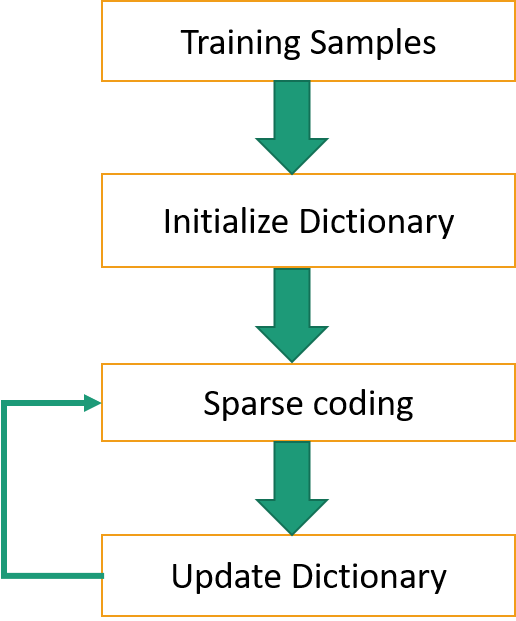
\includegraphics[width=.22\textheight]{figures/DLpipeline}
\linebreak
\caption{Pipeline of basic dictionary learning and sparse coding.}
\label{fig1:DLSC}
\end{figure}

\section{Joint Transfer and Dictionary Learning Framework}

The JDTL paradigm is shown in Figure~\ref{fig1:JLP}. The left-hand side of the figure is the generic transfer learning modeling where different views features are brought into common subspace using different transfer learning methods. While on the right-hand side we aim to learn view independent dictionary and coefficients by using the LRSDL~\cite{7987024} method. More detail is given in following subsections.

\begin{figure}[!ht]
	\centering
	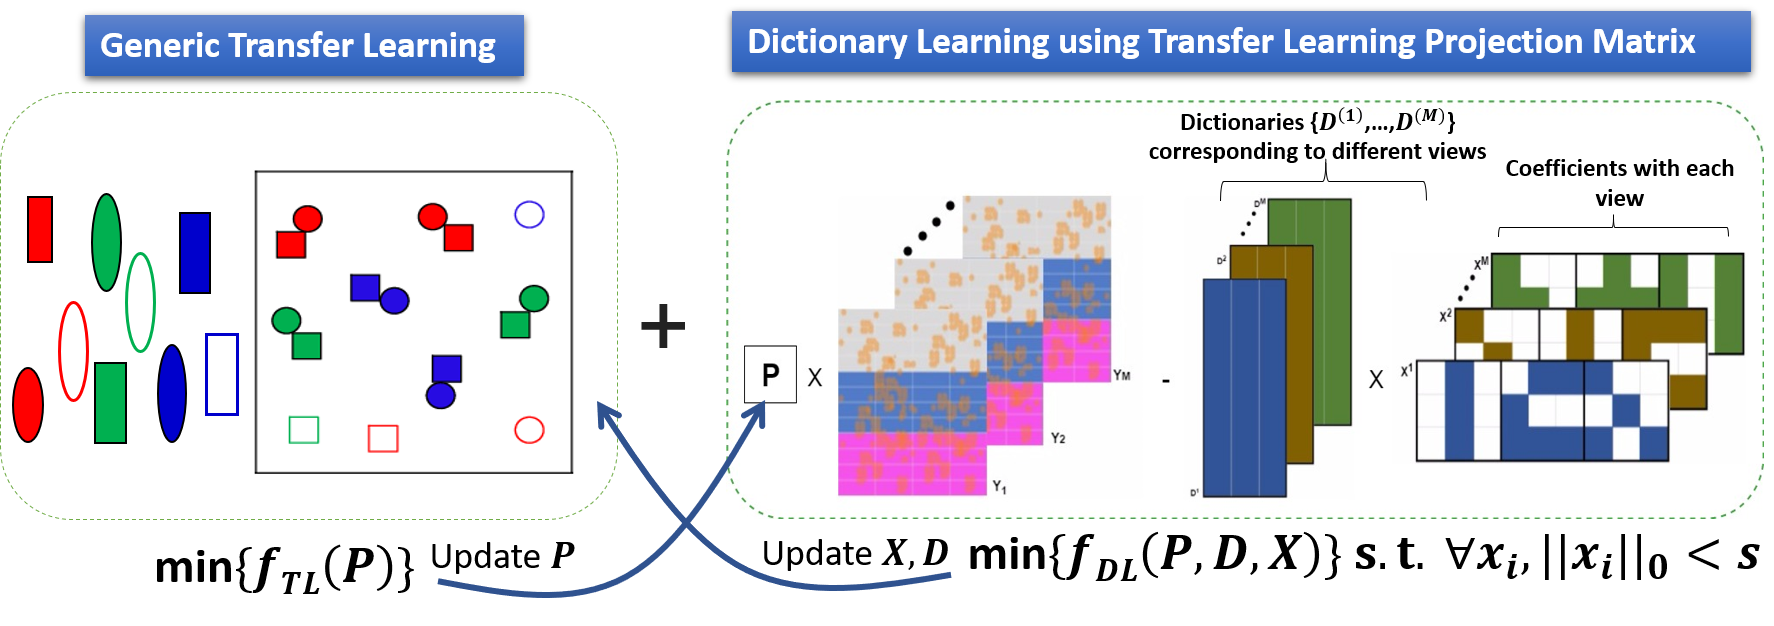
\includegraphics[width=.66\textheight]{figures/JLPara2}
	\linebreak
	\caption{Joint dictionary and transfer learning paradigm.}
	\label{fig1:JLP}
\end{figure}
\begin{figure}[!ht]
	\centering
	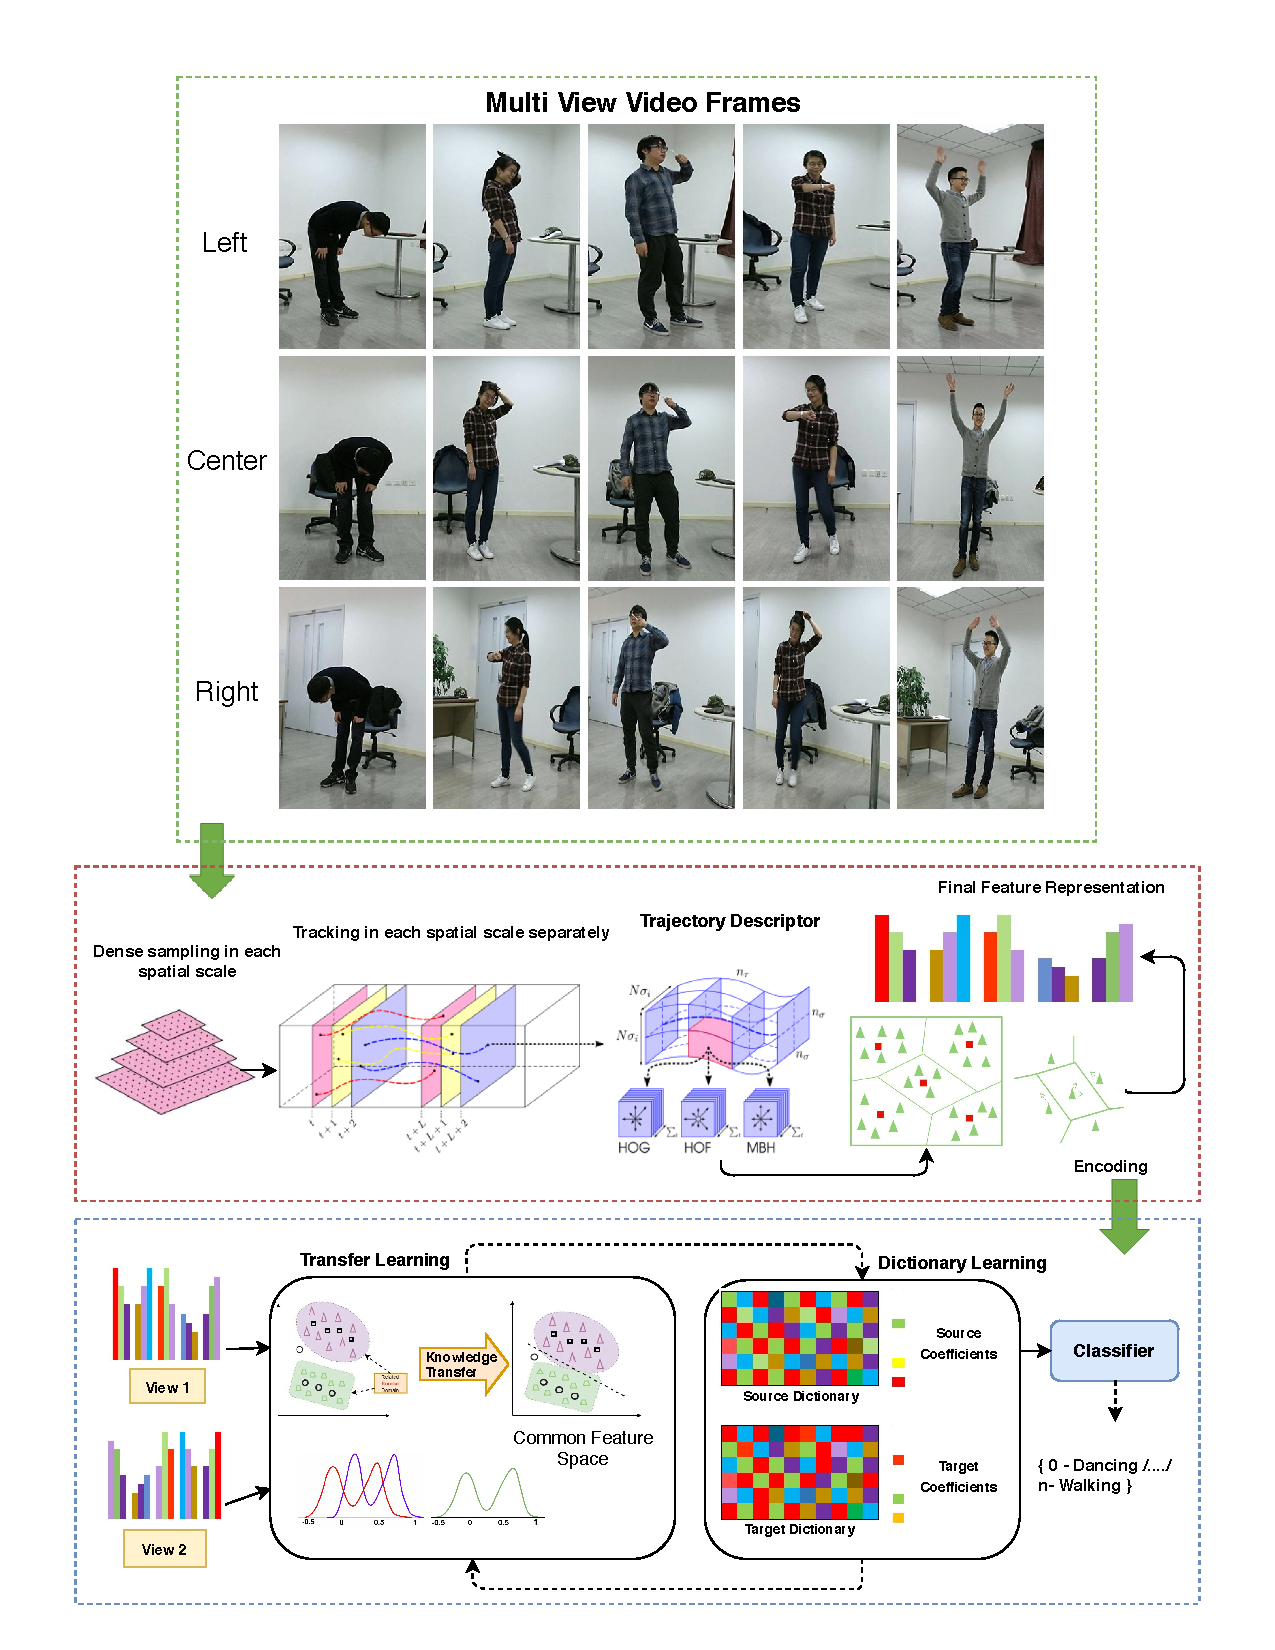
\includegraphics[width=.66\textheight]{figures/framework/updatewholepage2}
	\linebreak
	\caption{Overview of the proposed joint learning objective. Part of illustration is from~\cite{HengWang:2011:ARD:2191740.2192078}.}
	\label{fig1:JDTL}
\end{figure}
\subsection{Framework Overview}
The framework of our proposed method is shown in Figure~\ref{fig1:JDTL}. Where first we extract features from videos of each view using IDT method, then different transfer learning methods are used to bring features from different views into common subspace, and transfer learning projection matrix is learned. After learning the projection matrix, the view independent dictionary is learned. In the last, our novel approach is used to jointly learn the dictionary and projection matrix in order to get the optimized dictionary, coefficients and transfer learning projection matrix. Finally, SVM is used for the classification.

\subsection{Model Construction}
Let $Y$ be a set of $m$-dimensional training samples, i.e., $Y^{(v)} = [Y_1^{(v)}, Y_2^{(v)}, ....., Y_C^{(v)}]$ where $Y_i$ denotes the training sample from class $i$ and $C$ denotes the number of classes for each view. The view independent dictionary is denoted by $D^{(v)}= [D_1^{(v)}, D_2^{(v)},....,D_C^{(v)}]$ where $D_i$ is sub-dictionary associated with class $i$ and $v$ represents the views. In this approach we also learn the transfer learning projection matrix $P \in R^{m\times d}$, that projects the data into lower-dimensional space. $X^{(v)}$ is the sparse representation matrix of dimensionality reduced data $P^\T Y$ over dictionary $D^{(v)}$,
$f_{\text{TL}}(\cdot)$ is the transfer learning objective function which we get from different transfer learning methods, $f_{\text{DL}}(\cdot)$ is the general dictionary learning function. Hence, our proposed novel approach is given in the following equation:
\begin{equation}
\begin{aligned}
%\underset{D,X,P} \min = P_tY + ||P_{t-1}Y - D_{t-1}X_{t-1} ||
% & \min f(P) + ||P^\T Y - DX ||_F^2, \\
& \min_{P,D,X} f_{\text{TL}}(P) + \gamma f_{\text{DL}}(P,D,X), \\
\text{s.t. } & ||x_i||_0 < s \text{ and } x_i \text { is a column of } X,
\end{aligned}
\label{label:JDLTL}
\end{equation}
where $\gamma$ is the balancing parameter.


\subsection{Optimization}
The above equation can not be solved in closed form, so we refer to an iterative solution. The iterative process is shown in Figure~\ref{fig1:novelpipeline} and Algorithm~\ref{alg:JDTL}. Here our goal is to learn the projection matrix obtained via transfer learning and in the next step based on the projection matrix dictionary and sparse codes are updated.
The objective function in Eq.~\eqref{label:JDLTL} can be divided into three subproblems, to jointly learn projection $P$, dictionary $D$ and coding coefficients $X$.

\begin{figure}[!ht]
	\centering
	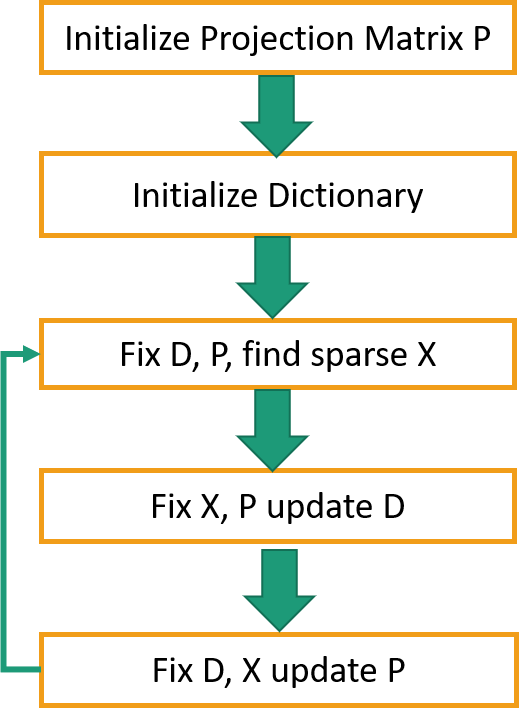
\includegraphics[width=.22\textheight]{figures/novelpipeline}
	\linebreak
	\caption{Pipeline of joint dictionary and transfer learning.}
	\label{fig1:novelpipeline}
\end{figure}  
\begin{algorithm}
	\caption{Joint Dictionary and Transfer Learning}
	\begin{algorithmic}[1]
		\State \textbf{Input}\\
		~~~Initialize $P_i$ as an output from transfer learning method.\\
		~~~Initialize $D_i$ and $X_i$ as a view independent Dictionary and Coefficients respectively 
		\While{convergence or maximal iteration step is not reached}
		\State $t \leftarrow t+1$
		\State Fix $P_i$ and $D_i$, update $X_i$  using \textbf{Equation:~\eqref{eq:DLX}}
		\State Fix $P_i$ and $X_i$, update $D_i$ using \textbf{Equation:~\eqref{eq:DL0}}
		\State Fix $D_i$ and $X_i$, update $P_i$  using \textbf{Equation:~\eqref{eq:DLPL}}
		\EndWhile\label{euclidendwhile}
		\State \textbf{output} $P, X$ and $D$
	\end{algorithmic}
\label{alg:JDTL}
\end{algorithm}
\noindent

First, different transfer learning methods are used to get the projection matrix. The projection matrix is learned by calculating the gradient of the projection matrix. Fast Low-Rank Shared Dictionary Learning (LRSDL) framework is used for the dictionary and coefficient learning. LRSDL method automatically extracts both discriminative and shared bases. LRSDL framework is a supervised method which learns a dictionary to extract the discriminative features for each class independently and also learns the shared features~\cite{7987024}. In our method shared dictionary and coefficients are used. FDDL has been broadly used for exploiting both structured dictionary and learning discriminative coefficient in LRSDL~\cite{612628612}. Specifically, the discriminative dictionary $D$ and the sparse coefficient matrix $X$ is learned based on the following equation.
\begin{equation}
\begin{aligned}
	J_Y(D,X) = \frac{1}{2}f_Y(D,X) + \lambda_1||X||_1 + \frac{\lambda_2}{2}g(X),
\end{aligned}
\label{eq:DL}
\end{equation}
where $f_Y(D,X) =  \sum\limits_{c=1}^{C} r_{Y_c}(D,X_c)$ is a discriminative fidelity with:
\begin{equation}
\begin{aligned}
r_{Y_c}(D,X_c) = ||Y_c-DX_c||_F^2 + ||Y_c - D_cX_c^c||_F^2 + \sum\limits_{j\neq c}||D_jX_c^j||_F^2.
\end{aligned}
\end{equation}

For $c = 1, \cdots,C$ ; $i =0,1,\cdots, C$. Assume that $Y_c \in \mathbb{R}^{d\times n_c}$ and $Y \in \mathbb{R}^{d \times N}$ with $N = \sum_{c=1}^{C}n_c$; $D_i \in \mathbb{R}^{d\times k_i} , D \in \mathbb{R}^{d\times K}\text{ with } K = \sum_{c=1}^{C}k_c $; and $X \in \mathbb{R}^{K \times N}$. Notation $X^i$ means the sparse coefficient of $Y$ on $D_i$, by $X_c \in \mathbb{R}^{K \times N_c}$ means the sparse coefficient of $Y_c$ on $D$ and by $X_c^i$ means the sparse coefficient of $Y_c$ on $D_i$.  

The last term in $r_{Y_c}(D,X_c)$ means that $D_j$ has small contribution to the representation of $Y_c$ for all $j\neq c$, and $g(X) = \sum_{c=1}^{C}(||X_c - M_c||_F^2 - ||M_c - M||_F^2) + ||X||_F^2 $. In $g(X)$, 
$M_c = \mu(X_c)$ and $M = \mu(X,n)$ is the mean matrices. $n$ is the number of columns depending on the context. The last term $||X||_F^2$ in $g(X)$ makes the cost function convex with respect to $X$. These subproblems are optimized alternatively by updating one variable and fixing the others, through an iterative process. Our proposed method is discussed in the following sections.

\subsection*{Updating Coding Coefficients $X$}

Assuming $D$ and $P$ are fixed, $X$ is solved by following equation:
\begin{equation}
\begin{aligned}
\min_X h(X) + \lambda ||X||_1,
\end{aligned}
\label{eq:DLX}
\end{equation}
where $h(X) = \frac{1}{2}f_{Y,D}(X) + \frac{\lambda_2}{2}g(X)$. This problem can be solved by FISTA~\cite{beck2009fast}. Where gradient of $f(\cdot)$ and $g(\cdot)$ are calculated with respect to $X$.
%Where we need to calculate gradient of $f(\cdot)$ and $g(\cdot)$ with respect to $X$. 
The gradient of $h(X)$ is calculated in FDDL method by the following equation: 
\begin{equation}
\begin{aligned}
\frac{\partial \frac{1}{2}f_{Y,D}(X)}{\partial X} = \mathcal{M}(D^\T D)X - \mathcal{M}(D^\T Y),
\end{aligned}
\label{eq:GRAD1}
\end{equation}
\begin{equation}
\begin{aligned}
\frac{\partial \frac{1}{2}g(X)}{\partial X} = 2X + M -2\underbrace{[M_1, M_2 ,.... , M_c]}_{\widehat{M}},
\end{aligned}
\label{eq:GRAD21}
\end{equation}
Where $\mathcal{M(\cdot)}$ doubles the diagonal block of the given matrix. The row and column partition of the matrix are inferred from the given matrix and it is also computationally inexpensive function of the given matrix . $\widehat{M}=[M_1, M_2 ,.... , M_c] = [\mu(X_1), \mu(X_2) ,.... , \mu(X_c)]$ is the mean of each class specific coefficients.

\noindent
Using Eq.~\eqref{eq:GRAD1} and Eq.~\eqref{eq:GRAD21} we obtain:
\begin{equation}
\begin{aligned}
\frac{\partial h(X)}{\partial X} = (\mathcal{M} (D^\T D) + 2 \lambda_2 I)X - \mathcal{M}(D^\T Y)+\lambda_2(M-2 \widehat{M}).
\end{aligned}
\label{eq:GRAD2}
\end{equation}

As the LRSDL is the extension of FDDL, class-specific coefficients $X$ and shared coefficients $X^0$ are solved alternatively, Here $X$ and $X^0$ are combined into one and find $\bar{X}$ by solving the following optimization problem:%  and will solve the optimization problem by the following equation:
\begin{equation}
\begin{aligned}
\bar{X} = \mathrm{arg}\ \underset{\bar{X}}{\min}\ {\bar{h}(\bar{X})} + \lambda_1 ||\bar{X}||_1.
\end{aligned}
\label{eq:GRAD3}
\end{equation}
where $\bar{h}(\bar{X}) = \frac{1}{2} \bar{f}_{Y,\bar{D}}(\bar{X}) + \frac{\lambda_2}{2}\bar{g}(\bar{X})$. This problem is solved using FISTA with the gradient of $\bar{h}(\bar{X})$:
\begin{equation}
\begin{aligned}
\bigtriangledown \bar{h}(\bar{X}) = 
\begin{bmatrix} \frac{\partial \bar{h}_{X^0}(X)}{\partial X} \\ \frac{\partial \bar{h}_{X}(X^0)}{\partial X^0} \end{bmatrix}.
\end{aligned}
\label{eq:GRAD4}
\end{equation}
\noindent
In the upper term, by combining the observations
\begin{equation}
\begin{aligned}
\bar{h}_{X^0}(X) & = \frac{1}{2}\bar{f}_{Y, \bar{D},X^0} (X) + \frac{\lambda_2}{2}\bar{g}_{X^0}(X)\\
& = \frac{1}{2}\bar{f}_{\bar{Y},{D}} (X) + \frac{\lambda_2}{2}{g}(X) + \text{constant},
\end{aligned}
\label{eq:GRAD5}
\end{equation}
where $\bar{D} = [D D_0]$ is total dictionary  and $\bar{Y} = Y - D_0X^0$ 
and using the equation, we have:
\begin{equation}
\begin{aligned}
\frac{\partial \bar{h}_{X^0}(X)}{\partial X} = (\mathcal{M} (D^\T D) + 2 \lambda_2 I)X - \mathcal{M}(D^\T \bar{Y})+\lambda_2(M-2 \widehat{M}).
\end{aligned}
\label{eq:GRAD6}
\end{equation}
the lower term is solved by 
\begin{equation}
\begin{aligned}
\bar{h}_X(X^0) = ||V-D_0X^0||_F^2 + \frac{\lambda_2}{2}||X^0 - M^0||_F^2 + \text{constant},
\end{aligned}
\label{eq:GRAD7}
\end{equation}
\begin{equation}
\begin{aligned}
\Rightarrow \frac{\partial \bar{h}_{X}(X^0)}{\partial X^0} & = 2D_0^TD_0X^0 - 2D_0^TV +\lambda_2(X^0 - M^0),\\
& = (2D_0^TD_0+\lambda_2I)X^0 - 2D_0^TV - \lambda_2M^0,
\end{aligned}
\label{eq:GRAD8}
\end{equation}
where $V = Y-\frac{1}{2}D\mathcal{M}(X)$ and $X^0$ is the shared coefficients and $M^0$ is the mean vector of shared coefficients. The Eq.~\eqref{eq:GRAD4} can be solved by combining Eq.~\eqref{eq:GRAD8} and Eq.~\eqref{eq:GRAD6}.
%So combining Eq.~\eqref{eq:GRAD8} and~\eqref{eq:GRAD6}, the Eq.~\eqref{eq:GRAD4} can be solved.
After solving the equation, $\bigtriangledown \bar{h}(\bar{X})$, $\bar{X}$ can be updated by FISTA algorithm. We also need to compute the Lipschitz coefficient $L$ of $\bigtriangledown \bar{h}(\bar{X})$.


\subsection*{Updating Dictionary $D$}

$D$ is updated by fixing $P$ and $X$. 
The most important part of the shared dictionary is to represent samples from all classes. In other words,
it is expected that the collaboration of the particular dictionary $D_c$ and the shared dictionary $D_0$ should well represent $Y_c$. 
 %it is expected that $Y_c$ can be well represented by the collaboration of the particular dictionary $D_c$ and shared dictionary $D_0$. 
 The discriminative fidelity term $f_Y(D,X)$ in Eq.~\eqref{eq:DL} can be extended to $\bar{f}_Y(\bar{D},\bar{X}) = \sum_{c=1}^{C}\bar{r}_{Y_c}(\bar{D},\bar{X_c})$ with $\bar{r}_{Y_c}(\bar{D},\bar{X_c})$ is defined as:
%This above approach can be solved by the following equation:
\begin{equation}
\begin{aligned}
||Y_c-\bar{D}\bar{X_{c}}||_F^2 + ||Y_c-D_c X_c^c-D_0X_c^0||_F^2 + \sum_{j=1,j\neq c} ||D_jX_c^j||_F^2.
\end{aligned}
\label{eq:DL0}
\end{equation}
Since $\bar{r}_{Y_c}(\bar{D},\bar{X_c}) = r_{\bar{Y}_c}(D,X_c)$ with $\bar{Y}_c = Y_c-D_0X_c^0$, we have $\bar{f}_Y(\bar{D},\bar{X}) = f_{\bar{Y}}(D,X)$ with $\bar{Y}=Y-D_0X^0$

The atoms that are the part of shared dictionary $D_0$ should represent the samples from all classes. The nuclear norm regularization $||D||_*$ is used as a convex relaxation of $D_0$. It forces that shared dictionary should have low-rank to prevent the dictionary from absorbing the discriminative atoms and it handles the worst case, where all atoms are the part of shared dictionary and there is no discriminative features remaining for class-specific atoms.

The contribution of each class-specific feature might be different, even the shared dictionary has low-rank. The contribution of each class-specific feature is measure by shared coefficients $X_0$, which they aim to avoid. A regularization term $||X^0 - M^0||$ is added that forces each $x^0$ to be close to mean vector $m^0$ for all $X^0$. By adding this constraint, the fisher-based discriminative coefficient term $g(x)$ can be extended to $\bar{g}(\bar{x})$ and it is defined as:
\begin{equation}
\begin{aligned}
	\bar{g}(\bar{x}) = g(X) +||X^0-M^0||_F^2,
	\end{aligned}
	\label{extendg(x)}
\end{equation}
In total, the cost function $\bar{J}_Y(\bar{D},\bar{X})$ of the LRSDL method is: 
\begin{equation}
\begin{aligned}
\bar{J}_Y(\bar{D},\bar{X}) = \frac{1}{2}\bar{f}_Y(\bar{D},\bar{X})+\lambda_1||\bar{X}||_1 + \frac{\lambda_2}{2}\bar{g}(\bar{X}) + \eta||D^0||_*.
\end{aligned}
\label{lrsdlcostfunction}
\end{equation}
The shared dictionary and class-specific dictionary can be found by minimizing the objective function. $\bar{D}, \bar{X}$ become $D, X$ respectively, $\bar{J}_Y(\bar{D},\bar{X})$ becomes $J_Y({D},{X})$ and LRSDL reduces to FDDL in case if there is no shared dictionary.

The FDDL method updates each class-specific dictionary by fixing the $X$. This process takes time for convergence, so in LRSDL the total dictionary $D$ is optimized while fixing $X$ instead of updating the class-specific dictionaries, so this problem is given in below equation:
\begin{equation}
\begin{aligned}
\min_D \ f_{Y,X}(D) \Rightarrow \min_D\big\{-2 \textbf{tr}(ED^\T) +\textbf{tr}(FD^\T D)\big\},
\end{aligned}
\label{eq:DL1}
\end{equation}
where $E= Y \mathcal{M}(X^\T) $, \textbf{tr($\cdot$)} means the trace of a matrix, and \textcolor{blue}{${F}$}$ = \mathcal{M}(XX^\T)$.

The LRSDL method finds total dictionary $\bar{D} = [D, D_0]$. So, the method solves the $D$ and $D_0$ separately. First, to update the $D$ in Eq.~\eqref{eq:DL0}, assuming $\bar{f}_y(\bar{D}, \bar{X}) = f_Y(D,X) $ with $\bar{Y} \triangleq Y_ {D_0}X^0$, the E-FDDL-D algorithm for $D$ is similar to Eq.~\eqref{eq:DL1}. Second, $D_0$ is optimized through the following equation when $D, X$ in Eq.~\eqref{lrsdlcostfunction} are fixed,
\begin{equation}
\begin{aligned}
\bar{J}_{Y,D,X}(D_0,X_0) = & ||V-D_0X_0||_F^2 + \frac{\lambda_2}{2} ||X^0 - M^0||_F^2 + \\ 
 & \eta||D_0||_* + \lambda_1||X^0||_1 + \text{constant},\\
\end{aligned}
\label{eq:DL4}
\end{equation}
and $V = Y- \frac{1}{2}D\mathcal{M}(X)$. 
The $D_0$ is updated by solving following equation based on the above equation:
\begin{equation}
\begin{aligned}
\min_{D_0} \ \textbf{tr}(FD_0^\T D_0) -2 \textbf{tr}(ED_0^\T)+ \eta ||D_0||_*,
\end{aligned}
\label{eq:DL5}
\end{equation}
where $E=V(X^0)^T$ ; $F = X^0(X^0)^T$ using the ADMM~\cite{boyd2011distributed36} method and singular value thresholding algorithm~\cite{cai2010singular}. In ADMM process we choose $\rho$ that should be greater than 0 and $Z = U = D_0$ is initialized, then the following problems are solved alternatively until they meet convergence.
\begin{equation}
\begin{aligned}
& \min_{D_0} - 2\textbf{tr}(\bar{E}D_0^\T) + \textbf{tr}(\bar{F}D_0^\T D_0), \\
& \text{with }\bar{E} = E+\frac{\rho}{2}(Z-U);  \bar{F} = F+\frac{\rho}{2}I,\\
\end{aligned}
\label{D0update}
\end{equation}
\begin{equation}
\begin{aligned}
Z = \mathcal{D_{\eta/\rho}}(D_c+U),
\end{aligned}
\label{Zeq}
\end{equation}
where $\mathcal{D}$ is shrinkage thresholding operator~\cite{cai2010singular}.
\begin{equation}
\begin{aligned}
U = U+D_0-Z.
\end{aligned}
\label{Ueq}
\end{equation}
The Eq.~\eqref{D0update} can be solved by ODL~\cite{mairal2010online} and the Eq.~\eqref{Zeq} and Eq.~\eqref{Ueq} are computationally inexpensive.

\subsection*{Updating Projection $P$}
First different transfer learning methods are used to get the projection matrix. Then, we minimize the projection matrix by calculating the gradient of the projection matrix. The projection matrix is optimized by using the similar way as sparse coefficients $X$ are optimized. Here, we used the FDDL method to optimize the projection matrix. 
\begin{equation}
\begin{aligned}
\min_P \frac{1}{2}f_{Y,D,X}(P) + \frac{\lambda_2}{2}g(P).
\end{aligned}
\label{eq:DLPL}
\end{equation}
This problem can be solved by FISTA, where we need to calculate gradient with respect to $P$. The gradients of the first and second terms can be calculated by FDDL method using the equations given below.   

\begin{equation}
\begin{aligned}
\frac{\partial \frac{1}{2}f_{Y,D}(P)}{\partial P} = \mathcal{M}(D^\T D)P - \mathcal{M}(D^\T (P^\T Y)),
\end{aligned}
\label{eq:PGRAD1}
\end{equation}
\begin{equation}
\begin{aligned}
\frac{\partial \frac{1}{2}g(P)}{\partial P} = 2P + M -2\underbrace{[M_1, M_2 ,.... , M_c]}_{\widehat{M}}.
\end{aligned}
\label{eq:PGRAD2}
\end{equation}
Using Eq.~\eqref{eq:PGRAD1} and~\eqref{eq:PGRAD2} we obtain:
\begin{equation}
\begin{aligned}
\frac{\partial h(P)}{\partial P} = (\mathcal{M} (D^\T D) + 2 \lambda_2 I)P - \mathcal{M}(D^\T (P^\T Y))+\lambda_2(M-2 \widehat{M}).
\end{aligned}
\label{eq:GRAD245}
\end{equation}







